\newpage \section{Analyse des opportunités des technologies libre dans
le domaine de l'édition vidéo et prévisions}

\paragraph{} Maintenant que les besoins et que les solutions existantes
ont été analysées dans le détail on se doit de rendre compte de la
situation actuel des technologies libres, de leurs communautés. Il est
aussi important de chercher les raisons qui expliquent le fait que ces
logiciels ne sont pas utilisés par les professionnels et trouver les
solutions possibles qui permettrais de remédier à ce fait.

\paragraph{} Dans cette partie, nous analyseront la différence entre les
manière d'envisager la création de logiciel, verrons quels sont les
avantages et inconvénients de ces fonctionnements. Par la, suite nous
nous concentrerons sur les frameworks existants pour faire une analyse
technique profonde des ces technologies. Par la suite, nous analyserons
les communauté qui portent ces différents projets afin d'arriver à
voir les lacunes et les avantages de chacun des projets.  Pour finir,
nous tirerons les conclusions de cette analyse afin de trouver des
solutions aux défis qu'est la création d'un logiciel libre de montage
vidéo. Mais pour commencer il est nécessaire d'analyser l'état de
l'art en terme de logiciel à proprement parler.

\subsection{Etat de l'art}

La création d'un logiciel open source d'édition vidéo, a été un
objectif pour de nombreux projet logiciel. Du fait de la complexité
inhérente au montage de vidéo de manière non linéaire, peu de projet
ont pu durée afin de murir et être réellement utilisable par les
utilisateurs comme le montre schéma suivant:

\newpage
\begin{figure}
  \begin{center}
    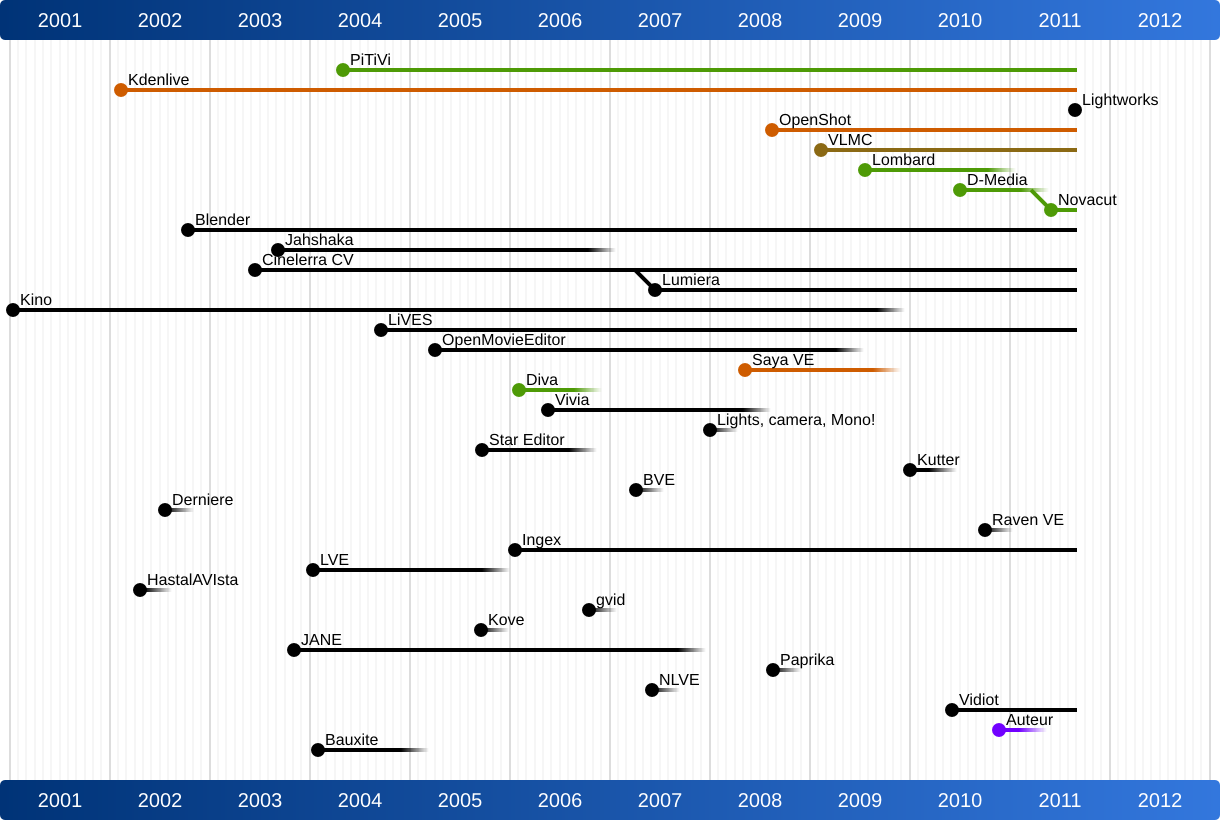
\includegraphics[width=0.9\textwidth]{images/open-source-video-editor-timeline}
  \end{center} \caption{Open source video editors timeline} \label{Yes}
\end{figure}

\paragraph{} A l'heure actuel, il existe un nombre réduit de projet qui
sont plus ou moins mature, mais des projet issue du monde propriétaire
sont en train de faire la transition vers la libération de leur code
\cite{TheLightworksOpenSourceProjectStartHere}. Cela fait plus d'un an que
le projet de libération de lightworks a été lancé mais la libération
du code n'a toujours pas eu lieu. Il ne sera donc pas possible d'analyser
le produit de manière technique, et il conviendra de le faire au moment
ou le code sera effectivement publiquement visible.

\subsection{Technologies} \paragraph{} Pour faire une analyse technique
des produits permettant de faire de l'édition vidéo, il est nécessaire
d'analyser en profondeur le core des logiciels, c'est à dire la partie du
logiciel où les operations d'édition sont effectivement réalisé. Dans
ce domaines, il existe 2 façon de procéder dans le monde de l'édition
vidéo open source.

\begin{itemize}
  \item{La première est de réaliser à la fois la partie graphique et
    les calculs permettant la gestion de l'édition non linéaire au
    sein d'une même entité de code. Le résultat de celà est un logiciel
    monolithiques. Le logiciel Cinelerra est un %FIXME
    example dans lequel les développeurs ont décidés d'utiliser ce
    mode de fonctionnement.}
  \item{La deuxième est d'utiliser/créer un framework\footnote{Un
    framework est un ensemble d'outils et de composants logiciels
    organisés conformément à un plan d'architecture et des design
    patterns. L'ensemble forme un squelette de programme.}, et d'ensuite
    créer une interface graphique utilisant ce cadre logiciel. La
    plupart des logiciels libre ont suivi ce plan de conception. Le
    logiciel PiTiVi utilise le Framework multimedia GStreamer alors que
    KDEnlive utilise le framework orienté édition et broadcasting
    MLT. Dans le cadre des Frameworks, nous nous intéresserons en
    particulier à l'analyse de ceux-ci puisque les notions relative à
    l'édition vidéo, et la gestion de toute la partie multimédia est
    réalisé par ceux-ci. Les logiciels d'édition ne sont à priori
    que de simples interfaces graphiques basé sur ces frameworks,
    et par conséquent leur analyse ne présente qu'un faible intérêt.}
\end{itemize}

\subsubsection{Logiciel monolithiques} %FIXME Look for a def

\paragraph{} Par le terme technologies intégrer, il convient de
comprendre que le logiciel peu utiliser des libraries externe, mais
le core de ce même logiciel, et la logique d'édition linéaire à
proprement parlé est directement faite à l'intérieur du logiciel et
non par une librairie, framework externe. Cela a pour principal avantage
que la conception est simplifié pour plusieurs raisons à savoir:

\begin{itemize}
  \item {Les développeurs n'ont pas la nécessité de penser
    en terme d'API, et n'ont pas à garantir la stabilité de
    celle-ci. Cela à pour effet que la qualité de l'architecture
    risque de ne pas être optimal puisque la création d'API force
    les développeurs/architectes à réellement analyser les besoins
    en profondeur dès le début et dans le cadre ou l'on ne crée pas
    %FIXME citations d'interface publique de programmation voué à
    être réutilisé, le risque est que ce travail ne soit pas fait.}
  \item {Les développeurs n'ont besoin de penser l'architecture, pour
    les seuls cas d'utilisation qui sont liés à ce même logiciel, %FIXME citations 
    ils n'ont pas à voir au delà de ces use cases.}
  \item {Les erreur en termes de design n'on}
\end {itemize}

\paragraph{} On se rend compte que cette amnière de faire a pour
principale avantage le fait que le logiciel peu être développé plus
rapidement puisque le core du logiciel, et donc le code qui implémente
la logique de l'édition non linéaire est conçue avec pour seul cas
d'utilisation, celui du logiciel. Mais l'on peu se rendre compte que de
nombreux inconvénient existent de par la nature monolithique du design:

\begin{itemize}
  \item{TODO}
\end{itemize}

\paragraph{} De plus, afin d'implémenter un logiciel de montage vidéo
dans son ensemble, le de code à produire est considérable, comme
le montre les statistique (Annexes 2), le logiciel Cinelerra à lui
seul fait plus de 1 million de lignes. Une tel quantité de code est
difficile à maintenir et requiert des ressources importantes en terme
de main d'oeuvre.

\paragraph{} L'un des inconvénients de cette manière de faire est que
le code que l'on a à l'intérieur du logiciel n'est pas réutilisable
directement par d'autre projets, et par conséquent, on peut considérer
que cela est ``individualiste``, chose qu'il convient d'éviter dans le
cadre du développement de logiciel libre afin de ne pas dupliquer les
efforts, et le code.

\paragraph{} Cette façon de faire a été utilisé par le projet
Cinelerra, ce projet est le plus avancé en terme de fonctionnalité
que le marché des logiciels libre de montage ai à offrir. On peut
penser que le fait qu'il est le seul à avoir utiliser cette méthode
de l'intégration de tout le code au sein du logiciel peu expliquer ce
fait. Bien qu'il y ai évidemment de nombreux autre facteurs.


\subsubsection{Analyse technique}

\subsubsection{Analyse des communauté}

\subsection{Lacunes}

\subsection{Solution possibles}
